\documentclass[10pt,t]{beamer}


\setbeamersize{text margin left=10pt,text margin right=10pt}
\usetheme{lehigh}

\usefonttheme{professionalfonts}
\usefonttheme{serif}

% add packages to use
\usepackage{tabularx}
\usepackage{tikz}
\usetikzlibrary{trees,matrix,shapes,arrows}
\usetikzlibrary{calc}
\usepackage{fancyvrb}
\usepackage{listings}

\pgfdeclarelayer{background}
\pgfdeclarelayer{foreground}
\pgfsetlayers{background,main,foreground}
\usepackage[latin1]{inputenc}
\usepackage[english]{babel}
\usepackage{hyperref}
\usepackage[normalem]{ulem}

                                                         
%\usepackage{times}
%\usepackage[T1]{fontenc}
\usepackage{graphicx}
%\usepackage{pgf,pgfarrows,pgfnodes,pgfautomata,pgfheaps,pgfshade}
\usepackage{amsmath,amssymb,amsfonts,subfigure,pifont}
\usepackage{multirow}
\usepackage{booktabs}
\usepackage{colortbl}
\usepackage{keystroke}
\usepackage{etex}


% The following color are for listing environment 
\definecolor{dkgreen}{rgb}{0,0.6,0}
%\definecolor{gray}{rgb}{0.5,0.5,0.5}
\definecolor{mauve}{rgb}{0.58,0,0.82}


\lstset{%
language=bash,                % the language of the code
basicstyle=\tiny\ttfamily,           % the size of the fonts that are used for the code
showspaces=false,               % show spaces adding particular underscores
showstringspaces=false,         % underline spaces within strings
showtabs=false,                 % show tabs within strings adding particular underscores
%frame=single,                   % adds a frame around the code
%rulecolor=\color{black},        % if not set, the frame-color may be changed on line-breaks within not-black text (e.g. comments (green here))
tabsize=2,                      % sets default tabsize to 2 spaces
%captionpos=b,                   % sets the caption-position to bottom
breaklines=true,                % sets automatic line breaking
breakatwhitespace=false,        % sets if automatic breaks should only happen at whitespace
%title=\lstname,                   % show the filename of files included with \lstinputlisting;
% also try caption instead of title
keywordstyle=\color{blue},          % keyword style
commentstyle=\color{dkgreen},       % comment style
stringstyle=\color{mauve},         % string literal style
escapeinside={!}{!},            % if you want to add LaTeX within your code
morekeywords={*,\dots,elif},              % if you want to add more keywords to the set
deletekeywords={\dots},              % if you want to delete keywords from the given language
%morecomment=[l]{//}
}
\lstset{%
language=csh,                % the language of the code
basicstyle=\tiny\ttfamily,           % the size of the fonts that are used for the code
showspaces=false,               % show spaces adding particular underscores
showstringspaces=false,         % underline spaces within strings
showtabs=false,                 % show tabs within strings adding particular underscores
%frame=single,                   % adds a frame around the code
%rulecolor=\color{black},        % if not set, the frame-color may be changed on line-breaks within not-black text (e.g. comments (green here))
tabsize=2,                      % sets default tabsize to 2 spaces
captionpos=b,                   % sets the caption-position to bottom
breaklines=true,                % sets automatic line breaking
breakatwhitespace=false,        % sets if automatic breaks should only happen at whitespace
%title=\lstname,                   % show the filename of files included with \lstinputlisting;
% also try caption instead of title
keywordstyle=\color{blue},          % keyword style
commentstyle=\color{dkgreen},       % comment style
stringstyle=\color{mauve},         % string literal style
escapeinside={\%*}{*)},            % if you want to add LaTeX within your code
morekeywords={*,\dots,elif},              % if you want to add more keywords to the set
deletekeywords={\dots},              % if you want to delete keywords from the given language
%morecomment=[l]{//}
}

\lstdefinestyle{LINUX}
{
    backgroundcolor=\color{white},
    basicstyle=\tiny\ttfamily,
    keywordstyle=\color{blue},
    morekeywords={apacheco,Tutorials,BASH,scripts,day1,examples},
    literate={>}{{\textcolor{blue}{>}}}1
         {/}{{\textcolor{blue}{/}}}1
         {./}{{\textcolor{black}{./ }}}1
         {~}{{\textcolor{blue}{\textasciitilde}}}1,
}



\DeclareSymbolFont{extraup}{U}{zavm}{m}{n}
%\DeclareMathSymbol{\vardiamond}{\mathalpha}{extraup}{87}
\newcommand{\cmark}{\ding{51}}
\newcommand{\xmark}{\ding{55}}
\newcommand{\smark}{\ding{77}}
\newcommand*\vardiamond{\textcolor{lubrown}{%
  \ensuremath{\blacklozenge}}}
\newcommand*\mybigstar{\textcolor{lubrown!90!yellow}{%
  \ensuremath{\bigstar}}}
\newcommand*\up{\textcolor{green!80!black}{%
  \ensuremath{\blacktriangle}}}
\newcommand*\down{\textcolor{red}{%
  \ensuremath{\blacktriangledown}}}
\newcommand*\const{\textcolor{darkgray}%
  {\textbf{--}}}
\newcommand*\enter{\tikz[baseline=-0.5ex] \draw[<-] (0,0) -| (0.5,0.1);}

\newcommand{\Verblubrown}[1]{\Verb[formatcom=\color{lubrown},fontseries=b,commandchars=\\\{\}]|#1|}
\newcommand{\Verblue}[1]{\Verb[formatcom=\color{lublue},fontseries=b,commandchars=\\\{\}]!#1!}
\newcommand{\Verbblue}[2][b]{\Verb[formatcom=\color{lublue},fontshape=#1,commandchars=\\\{\}]|#2|}
\newcommand{\Verblubrownp}[1]{\Verb[formatcom=\color{lubrown},fontseries=b,commandchars=\\\{\}]!#1!}


% LOGOS
% footer logo
\pgfdeclareimage[width=0.3\paperwidth]{university-logo}{lulogo}
\tllogo{\pgfuseimage{university-logo}}

%titlepage logo
\titlegraphic{\includegraphics[scale=0.5]{lu}}


\beamertemplateballitem
\usetikzlibrary{mindmap,trees}
\usetikzlibrary{decorations.text,calc,arrows.meta}
\usepackage{tabu}

\newcolumntype{a}{>{\columncolor{lulime}}c}
\newcolumntype{b}{>{\columncolor{lulime!50}}c}
\newcolumntype{d}{>{\columncolor{lulime!40}}c}
\newcolumntype{e}{>{\columncolor{lulime}}l}
\newcolumntype{f}{>{\columncolor{lulime!50}}l}

\title{Shell Scripting}
%\subtitle{Variables, Arrays \& Control Constructs}
\author{Alexander B. Pacheco}
\institute{\href{http://researchcomputing.lehigh.edu}{LTS Research Computing}}%\\[2pt] \href{http://www.lehigh.edu}{Lehigh University}}
\date{ }
%\date{September 29 2015}%\today}

% Delete this, if you do not want the table of contents to pop up at
% the beginning of each subsection:
\AtBeginSection[]
{
  \begingroup
  \setbeamertemplate{background canvas}[vertical shading][bottom=lubrown,top=lubrown]
  \setbeamertemplate{footline}[myfootline] 
  \setbeamertemplate{section page}[mysection]
  \frame[c]{
    \sectionpage
  }
  \endgroup
}

\begin{document}

\begin{frame}
  \titlepage
\end{frame}

\footnotesize
\begin{frame}{Outline}
  \tableofcontents
\end{frame}

\section{Introduction}
\begin{frame}[label=day1]
  \frametitle{Introduction}
  \begin{exampleblock}{What is a SHELL}
    \begin{itemize}
      \item The command line interface is the primary interface to Linux/Unix operating systems.
      \item Shells are how command-line interfaces are implemented in Linux/Unix.
      \item Each shell has varying capabilities and features and the user should choose the shell that best suits their needs.
      \item The shell is simply an application running on top of the kernel and provides a powerful interface to the system.
    \end{itemize}
  \end{exampleblock}
  \begin{center}
    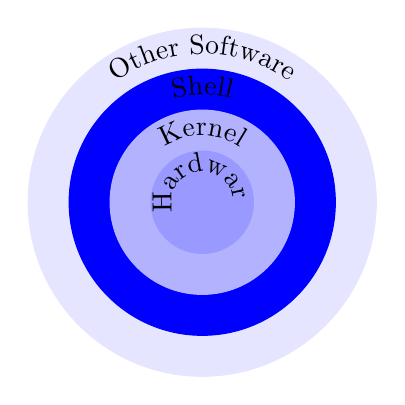
\begin{tikzpicture}[scale=0.65]
      \coordinate (O) at (0,0);
      \draw[fill=blue!10,blue!10] (O) circle (3.4);
      %\onslide<4>{\draw[fill=blue,blue] (O) circle (3.4);}
      \draw[fill=blue,blue] (O) circle (2.6);
      %\onslide<3>{\draw[fill=blue,blue] (O) circle (2.6);}
      \draw[fill=blue!30,blue!30] (O) circle (1.8);
      %\onslide<2>{\draw[fill=blue,blue] (O) circle (1.8);}
      \draw[fill=blue!40,blue!40] (O) circle (1.0);

      \draw[decoration={text along path,reverse path,text
align={align=center},text={Other Software}},decorate] (2.9,0) arc (0:180:2.9);
      \draw[decoration={text along path,reverse path,text
align={align=center},text={Shell}},decorate] (2.1,0) arc (0:180:2.1);
      \draw[decoration={text along path,reverse path,text
align={align=center},text={Kernel}},decorate] (1.3,0) arc (0:180:1.3);
      \draw[decoration={text along path,reverse path,text
align={align=center},text={Hardware}},decorate] (0.6,0) arc (0:180:0.6);
    \end{tikzpicture}
  \end{center}
\end{frame}

\subsection{Types of Shell} 
\begin{frame}
  \frametitle{Types of Shell}
  \begin{itemize}
    \item[\texttt{sh}]: Bourne Shell
      \begin{enumerate}
      \item[$\vardiamond$] Developed by Stephen Bourne at AT\&T Bell Labs
      \end{enumerate}
    \item[\texttt{csh}]: C Shell
      \begin{enumerate}
      \item[$\vardiamond$] Developed by Bill Joy at University of California, Berkeley
      \end{enumerate}
    \item[\texttt{ksh}]: Korn Shell
      \begin{enumerate}
      \item[$\vardiamond$] Developed by David Korn at AT\&T Bell Labs
      \item[$\vardiamond$] backward-compatible with the Bourne shell and includes many features of the C shell
      \end{enumerate}
    \item[\texttt{bash}]: Bourne Again Shell
      \begin{enumerate}
      \item[$\vardiamond$] Developed by Brian Fox for the GNU Project as a free software replacement for the Bourne shell (sh).
      \item[$\vardiamond$] Default Shell on Linux and Mac OSX
      \item[$\vardiamond$] The name is also descriptive of what it did, bashing together the features of sh, csh and ksh
      \end{enumerate}
    \item[\texttt{tcsh}]: TENEX C Shell
      \begin{enumerate}
      \item[$\vardiamond$] Developed by Ken Greer at Carnegie Mellon University 
      \item[$\vardiamond$] It is essentially the C shell with programmable command line completion, command-line editing, and a few other features.
      \end{enumerate}
  \end{itemize}
\end{frame}

\begin{frame}[c]
  \frametitle{Shell Comparison}
  \begin{center}
    \taburulecolor{lublue}
    \begin{tabular}{a|b|b|b|b|b}
      \rowcolor{lublue} & \textbf{sh} & \textbf{csh} & \textbf{ksh} & \textbf{bash} & \textbf{tcsh} \\
       Programming Language & \cmark & \cmark & \cmark & \cmark & \cmark \\
       Shell Variables & \cmark & \cmark & \cmark & \cmark & \cmark \\
       Command alias & \xmark & \cmark & \cmark & \cmark & \cmark \\
       Command history & \xmark & \cmark & \cmark & \cmark & \cmark \\
       Filename completion & \xmark & \smark & \smark & \cmark & \cmark \\
       Command line editing & \xmark & \xmark & \smark & \cmark & \cmark \\
       Job control & \xmark & \cmark & \cmark & \cmark & \cmark \\
    \end{tabular}
    \begin{columns}
      \column{0.6\textwidth}
      \begin{itemize}
      \item[\cmark]: Yes
      \item[\xmark]: No
      \item[\smark]: Yes, not set by default
      \item[] {\fontsize{6}{7}\selectfont\url{http://www.cis.rit.edu/class/simg211/unixintro/Shell.html}}
      \end{itemize}
    \end{columns}
  \end{center}
\end{frame}

\subsection{Variables}
\begin{frame}[fragile,allowframebreaks]
  \frametitle{Variables}
  \begin{itemize}
    \item A variable is a named object that contains data used by one or more applications. 
    \item There are two types of variables, Environment and User Defined and can contain  a number, character or a string of characters.
    \item Environment Variables provides a simple way to share configuration settings between multiple applications and processes in Linux.
    \item As in programming languages like C, C++ and Fortran, defining your own variables makes the program or script extensible by you or a third party
    \item Rules for Variable Names
    \begin{enumerate}
        \item Variable names must start with a letter or underscore
        \item Number can be used anywhere else
        \item DO NOT USE special characters such as \texttt{@, \#, \%, \$}
        \item Case sensitive
        \item Examples
        \begin{itemize}
          \item Allowed: VARIABLE, VAR1234able, var\_name, \_VAR
          \item Not Allowed: 1VARIABLE, \%NAME, \$myvar, VAR@NAME 
        \end{itemize}
    \end{enumerate}
    \item To reference a variable, environment or user defined, you need to prepend the variable name with "\$" as in \$VARIABLE, \$PATH, etc.
    \item Its a good practice to protect your variable name within \{\dots\} such as \$\{PATH\} when referencing it. (We'll see an example in a few slides)
    \item Assigning value to a variable
    \begin{center}
      \taburulecolor{lublue}
          \begin{tabular}{a|b|b}
            \rowcolor{lublue}\textbf{Type} & \textbf{sh,ksh,bash} &\textbf {csh,tcsh}\\
            Shell & name=value & set name = value \\
            Environment & export name=value & setenv name value \\
        \end{tabular}
    \end{center}
    \item \textbf{sh,ksh,bash} THERE IS NO SPACE ON EITHER SIDE OF =
    \item \textbf{csh,tcsh} space on either side of = is allowed for the \texttt{set} command
    \item \textbf{csh,tcsh} There is no = in the \texttt{setenv} command
  \end{itemize}
\end{frame}

\subsection{File Permissions}
\begin{frame}[fragile, allowframebreaks]
  \frametitle{File Permissions}
  \begin{itemize}
    \item In *NIX OS's, you have three types of file permissions
    \begin{enumerate}
        \item read (r)
        \item write (w)
        \item execute (x)
    \end{enumerate}
    \item for three types of users
    \begin{enumerate}
        \item user
        \item group
        \item world i.e. everyone else who has access to the system
    \end{enumerate}
    \begin{exampleblock}{}
      \begin{tabular}{lllllllll}
        drwxr-xr-x. & 2 & user & user & 4096 & Jan & 28 & 08:27 & Public\\
        -rw-rw-r-\,-. & 1 & user & user & 3047 & Jan & 28 & 09:34 & README\\
      \end{tabular}
    \end{exampleblock}
    \item The first character signifies the type of the file
    \item[] \Verblubrown{d} for directory
    \item[] \Verblubrown{l} for symbolic link
    \item[] \Verblubrown{-} for normal file
    \item The next three characters of first triad signifies what the owner can do
    \item The second triad signifies what group member can do
    \item The third triad signifies what everyone else can do
      \begin{gather*}
        d\underbrace{rwx}_{u}\overbrace{r-x}^g\underbrace{r-x}_o
      \end{gather*}
    \item Read carries a weight of 4
    \item Write carries a weight of 2
    \item Execute carries a weight of 1
    \item The weights are added to give a value of 7 (rwx), 6(rw), 5(rx) or 3(wx) permissions. 
    \item \Verblubrown{chmod} is a *NIX command to change permissions on a file
    \item To give user rwx, group rx and world x permission, the command is
    \item[] \Verblubrown{chmod 751 filename}
    \item Instead of using numerical permissions you can also use symbolic mode
  \end{itemize}
  \begin{description}
    \item[u/g/o or a] user/group/world or all i.e. ugo
    \item[+/-] Add/remove permission
    \item[r/w/x] read/write/execute
  \end{description}
  \begin{itemize}
    \item Give everyone execute permission: 
    \item[] \Verblubrown{chmod a+x hello.sh }
    \item[] \Verblubrown{chmod ugo+x hello.sh}
    \item Remove group and world read \& write permission: 
    \item[] \Verblubrown{chmod go-rw hello.sh}
    \item Use the \Verblubrown{-R} flag to change permissions recursively, all files and directories and their contents.
    \item[] \Verblubrown{chmod -R 755 \$\{HOME\}/*}
    \item[] What is the permission on \$\{HOME\}?
  \end{itemize}
  \begin{exampleblock}{HPC Users}
    If you want to share your files with your colleagues
    \begin{enumerate}
      \item Make your home directory read accessible to the world
      \item[] \Verblubrown{chmod 755 \$\{HOME\}}
      \item[] \textsc{do not use the recursive -R flag}
      \item Change to your home directory and give read access to the directory that you want to share using the -R flag
    \end{enumerate} 
  \end{exampleblock}
\end{frame}

\subsection{Input and Output}
\begin{frame}[fragile,allowframebreaks]
  \frametitle{Input/Output}
  \begin{itemize}
    \item For reading input from screen/keyboard/prompt
    \item[]\textbf{bash} \Verblubrown{read}
    \item[]\textbf{tcsh} \Verblubrown{\$<}
    \item The \Verblubrown{read} statement takes all characters typed until the \Enter \,key is pressed and stores them into a variable.
    \item[]Syntax \Verbblue{read <variable name>}
    \item[]Example \Verbblue{read name\Enter}
    \item[] \Verbblue{\textit{Alex Pacheco}}
    \item \Verblubrown{\$<} can accept only one argument. If you have multiple arguments, enclose the \Verblubrown{\$<} within quotes e.g. \Verblubrown{"\$<"}
    \item[]Syntax: \Verbblue{set <variable> = \$<}
    \item[]Example: \Verbblue{set name = "\$<"\Enter}
    \item[] \Verbblue{\textit{Alex Pacheco}}
    \item In the above examples, the name that you enter in stored in the variable \texttt{name}.
    \newpage
    \item The command \Verblubrown{echo} is used for displaying output to screen 
    \item Use the \Verblubrown{echo} command to print the variable \texttt{name} to the screen
    \item[] \Verbblue{echo \$name\Enter}
    \item The \Verblubrown{echo} statement can print multiple arguments. 
    \item By default, \Verblubrown{echo} eliminates redundant whitespace (multiple spaces and tabs) and replaces it with a single whitespace between arguments. 
    \item To include redundant whitespace, enclose the arguments within double quotes
    \item[] \texttt{echo Welcome to HPC\quad\quad Training}\enter\, (more than one space between HPC and Training)
    \item[] \texttt{echo "Welcome to HPC\quad\quad Training"}\enter
    \item[] \texttt{read name\enter} or \texttt{set name = "\$<"\enter}
    \item[] \textit{Alex\quad\quad\quad Pacheco\enter}
    \item[] \texttt{echo \$name\enter}
    \item[] \texttt{echo "\$name"\enter}
    \framebreak
    \item You can also use the \textbf{printf} command to display output
    \item[]Syntax: \texttt{printf <format> <arguments>}
    \item[]Example: \texttt{printf "\$name"\enter}
    \item[] \texttt{printf "\%s$\backslash$n" "\$name"\enter}
    \item Format Descriptors
    \begin{enumerate}
        \item[\%s] print argument as a string
        \item[\%d] print argument as an integer
        \item[\%f] print argument as a floating point number
        \item[$\backslash$n] print new line
        \item[] you can add a width for the argument between the \% and \{s,d,f\} fields
        \item[] \%4s, \%5d, \%7.4f
    \end{enumerate}
    \item The \textbf{printf} command is used in \textbf{awk} to print formatted data (more on this later) 
  \end{itemize}
\end{frame}

\begin{frame}
  \frametitle{I/O Redirection}
  \begin{itemize}
    \item There are three file descriptors for I/O streams
    \begin{enumerate}
        \item STDIN: Standard Input
        \item STDOUT: Standard Output
        \item STDERR: Standard Error
    \end{enumerate}
    \item 1 represents STDOUT and 2 represents STDERR
    \item I/O redirection allows users to connect applications
    \begin{itemize}
      \item[$<$]: connects a file to STDIN of an application
      \item[$>$]: connects STDOUT of an application to a file
      \item[$> >$]: connects STDOUT of an application by appending to a file
      \item[$|$]: connects the STDOUT of an application to STDIN of another application.
    \end{itemize}
    \item Examples:
    \begin{enumerate}
      {\footnotesize
      \item write STDOUT to file: \texttt{ls -l > ls-l.out }
      \item write STDERR to file: \texttt{ls -l 2> ls-l.err }
      \item write STDOUT to STDERR: \texttt{ls -l 1>\&2 }
      \item write STDERR to STDOUT: \texttt{ls -l 2>\&1 }
      \item send STDOUT as STDIN: \texttt{ls -l | wc -l}
      }
    \end{enumerate}
  \end{itemize}
\end{frame}

\section{Shell Scripting}
\begin{frame}
  \frametitle{What is a scripting language?}
  \begin{exampleblock}{}%{What is a Scripting Language?}
    \begin{itemize}
      \item A \textbf{scripting language} or \textbf{script language} is a \emph{programming language} that supports the writing of \textbf{scripts}.
      \item \textbf{Scripting Languages} provide a higher level of abstraction than standard programming languages.
      \item Compared to programming languages, scripting languages do not distinguish between data types: integers, real values, strings, etc.
      \item Scripting Languages tend to be good for automating the execution of other programs.
      \begin{enumerate}
          \item[$\vardiamond$] analyzing data
          \item[$\vardiamond$] running daily backups
      \end{enumerate}
      \item They are also good for writing a program that is going to be used only once and then discarded.
      \item A \textbf{script} is a program written for a software environment that automate the execution of tasks which could alternatively be executed one-by-one by a human operator.
      \item The majority of script programs are ``quick and dirty'', where the main goal is to get the program written quickly.
    \end{itemize}
  \end{exampleblock}
\end{frame}

\subsection{Getting Started with Writing Simple Scripts}
\begin{frame}[fragile]
  \frametitle{Writing your first script}
  \vspace{-0.25cm}
  \begin{block}{Three things to do to write and execute a script}
    \begin{enumerate}
      \item Write a script
      \begin{itemize}
        \item A shell script is a file that contains ASCII text. 
        \item Create a file, \texttt{hello.sh} with the following lines 
      \end{itemize}
      \begin{lstlisting}[language=bash]
#!/bin/bash
# My First Script
echo "Hello World!"
      \end{lstlisting}
      \item Set permissions
      \begin{lstlisting}[style=LINUX]
~/Tutorials/BASH/scripts> chmod 755 hello.sh 
      \end{lstlisting}
      \item[] OR
      \begin{lstlisting}[style=LINUX]
~/Tutorials/BASH/scripts> chmod a+x hello.sh 
      \end{lstlisting}
      \item Execute the script
      \begin{lstlisting}[style=LINUX]
~/Tutorials/BASH/scripts> ./hello.sh 
Hello World!
      \end{lstlisting}
      \item If you do not set execute permission for the script, then
        \begin{lstlisting}[style=LINUX]
~/Tutorials/BASH/scripts> sh hello.sh
Hello World!
      \end{lstlisting}
    \end{enumerate}
  \end{block}
\end{frame}

\begin{frame}[fragile]
  \frametitle{Description of the script}
  \begin{itemize}
    \item My First Script
  \begin{lstlisting}[language=bash]
#!/bin/bash
# My First Script
echo "Hello World!"
  \end{lstlisting}
    \item The first line is called the "ShaBang'' line. It tells the OS which interpreter to use. In the current example, bash
    \item Other options are:
    \begin{enumerate}
        \item[$\vardiamond$] \texttt{sh\quad\,:   \#!/bin/sh}
        \item[$\vardiamond$] \texttt{ksh :  \#!/bin/ksh}
        \item[$\vardiamond$] \texttt{csh :  \#!/bin/csh}
        \item[$\vardiamond$] \texttt{tcsh: \#!/bin/tcsh}
    \end{enumerate}
    \item The second line is a comment. All comments begin with "\#".
    \item The third line tells the OS to print "Hello World!" to the screen.
  \end{itemize}
\end{frame}

\begin{frame}
  \frametitle{Special Characters}
  \begin{description}
    \item[\#:] starts a comment.
    \item[\$:] indicates the name of a variable.
    \item[$\backslash$:] escape character to display next character literally.
    \item[\{\quad\}:] used to enclose name of variable.
    \item[;] Command separator [semicolon]. Permits putting two or more commands on the same line.
    \item[;;] Terminator in a case option [double semicolon].
    \item[.] "dot" command [period]. Equivalent to source. This is a bash builtin.
    \item[\$?] exit status variable.
    \item[\$\$] process ID variable.
    \item[{[\quad]}] test expression
    \item[{[[\quad]]}] test expression, more flexible than [ ] 
    \item[{\$[\quad], ((\quad))}] integer expansion
    \item[$||$, \&\&, !] Logical OR, AND and NOT
  \end{description}

\end{frame}

\begin{frame}
  \frametitle{Quotation}
  \begin{itemize}
    \item Double Quotation \texttt{" "}
    \begin{itemize}
        \item Enclosed string is expanded ("\$", "/" and "`")
        \item Example: \texttt{echo "\$myvar"} prints the value of \texttt{myvar}
    \end{itemize}
    \item Single Quotation \texttt{' '}
    \begin{itemize}
        \item Enclosed string is read literally
        \item Example: \texttt{echo '\$myvar'} prints \texttt{\$myvar}
    \end{itemize}
    \item Back Quotation \texttt{` `}
    \begin{itemize}
        \item Used for command substitution
        \item Enclosed string is executed as a command
        \item Example: \texttt{echo `pwd`} prints the output of the \texttt{pwd} command i.e. print working directory
        \item In \textbf{bash}, you can also use \texttt{\$($\cdots$)} instead of \texttt{`$\cdots$`}
        \item[] e.g. \texttt{\$(pwd)} and \texttt{`pwd`} are the same
    \end{itemize}
  \end{itemize}
\end{frame}

\begin{frame}[fragile]{Example}
  \lstinputlisting[language=bash]{./scripts/day1/examples/quotes.sh}
  \begin{lstlisting}[basicstyle=\tiny\ttfamily,style=LINUX]
~/Tutorials/BASH/scripts/day1/examples> ./quotes.sh 
HI
Hello
$HI
Hello
$HI

HelloAlex
/home/apacheco/Tutorials/BASH/scripts/day1/examples
/home/apacheco/Tutorials/BASH/scripts/day1/examples
~/Tutorials/BASH/scripts/day1/examples>
  \end{lstlisting}
\end{frame}

\subsection{Arithmetic Operations}
\begin{frame}[fragile,allowframebreaks]
  \frametitle{Arithmetic Operations}
  \begin{itemize}
    \item You can carry out numeric operations on integer variables
%  \end{itemize}
  \begin{columns}
    \column{0.5\textwidth}
    \begin{center}
       \taburulecolor{lublue}
          \begin{tabular}{abb}
            \rowcolor{lublue}{\textbf{Operation} }& {\textbf{Operator}} & \\
            Addition & + & \\
            Subtraction & - & \\
            Multiplication & * & \\
            Division & / & \\
            Exponentiation & ** & (\textbf{bash} only)\\
            Modulo & \% & \\ 
        \end{tabular}
    \end{center}
  \end{columns}
%  \begin{itemize}
    \item Arithmetic operations in \textbf{bash} can be done within the \texttt{\$(($\cdots$))} or \texttt{\$[$\cdots$]} commands
    \begin{enumerate}
      \item[$\bigstar$] Add two numbers: \texttt{\$((1+2))}
      \item[$\bigstar$] Multiply two numbers: \texttt{\$[\$a*\$b]}
      \item[$\bigstar$] You can also use the \texttt{let} command: \texttt{let c=\$a-\$b}
      \item[$\bigstar$] or use the \texttt{expr} command: \texttt{c=`expr \$a - \$b`}
    \end{enumerate}
    \framebreak
    \item In \textbf{tcsh},
    \begin{enumerate}
      \item[$\bigstar$] Add two numbers: \texttt{@ x = 1 + 2}
      \item[$\bigstar$] Divide two numbers: \texttt{@ x = \$a / \$b}
      \item[$\bigstar$] You can also use the \texttt{expr} command: \texttt{set c = `expr \$a \% \$b`}
    \end{enumerate}
    \item Note the use of space
    \item[\textbf{bash}] space required around operator in the \texttt{expr} command
    \item[\textbf{tcsh}] space required between @ and variable, around = and numeric operators. 
    \item You can also use C-style increment operators
    \item[\textbf{bash}] \texttt{let c+=1} or \texttt{let c-{}-}
    \item[\textbf{tcsh}] \texttt{@ x -= 1} or \texttt{@ x++}
    \item[] \texttt{/=}, \texttt{*=} and \texttt{\%=} are also allowed.
    \item[\textbf{bash}]
    \item The above examples only work for integers.
    \item What about floating point number?
    \framebreak
    \item Using floating point in \textbf{bash} or \textbf{tcsh} scripts requires an external calculator like GNU \texttt{bc}.
    \begin{enumerate}
        \item[$\bigstar$] Add two numbers:
        \item[]\texttt{echo "3.8 + 4.2" | bc}
        \item[$\bigstar$] Divide two numbers and print result with a precision of 5 digits:
        \item[]\texttt{echo "scale=5; 2/5" | bc}
        \item[$\bigstar$] Call \texttt{bc} directly:
        \item[]\texttt{bc $<<<$ "scale=5; 2/5"}
        \item[$\bigstar$] Use \texttt{bc -l} to see result in floating point at max scale:
        \item[] \texttt{bc -l $<<<$ "2/5"}
    \end{enumerate}
    \item You can also use \textbf{awk} for floating point arithmetic. 
  \end{itemize}
\end{frame}

\subsection{Flow Control}
\begin{frame}
  \frametitle{Flow Control}
  \begin{itemize}
    \item Shell Scripting Languages execute commands in sequence similar to programming languages such as C, Fortran, etc.
    \item Control constructs can change the sequential order of commands.
    \item Control constructs available in \textbf{bash} and \textbf{tcsh} are
    \begin{enumerate}
%      {\scriptsize
        \item Conditionals: \texttt{if}
        \item Loops: \texttt{for, while, until}
        \item Switches: \texttt{case, switch}
%      }
    \end{enumerate}
  \end{itemize}
\end{frame}

\begin{frame}[fragile]
  \frametitle{\texttt{if} statement}
  \begin{itemize}
    \item An \texttt{if/then} construct tests whether the exit status of a list of commands is 0, and if so, executes one or more commands.
    \begin{columns}
      \column{5cm}
      \begin{exampleblock}{bash}
        \begin{lstlisting}[language=bash]
if [ condition1 ]; then
  some commands
elif [ condition2 ]; then
  some commands
else
  some commands
fi
        \end{lstlisting}
      \end{exampleblock}
      \column{5cm}
      \begin{block}{tcsh}
        \begin{lstlisting}[language=csh]
if ( condition1 ) then
  some commands
else if ( condition2 ) then
  some commands
else
  some commands
endif
        \end{lstlisting}
      \end{block}
    \end{columns}
  \item Note the space between \textit{condition} and "["\quad"]"
  \item \textbf{bash} is very strict about spaces.
  \item \textbf{tcsh} commands are not so strict about spaces.
  \item \textbf{tcsh} uses the \texttt{if-then-else if-else-endif} similar to Fortran.   
  \end{itemize}
\end{frame}

\begin{frame}
  \frametitle{Comparison Operators}
   \begin{center}
    \begin{tabular}{ab|b}
      \rowcolor{lublue}\multicolumn{3}{c}{Integer Comparison} \\
      \rowcolor{lublue}Operation & \textbf{bash} & \textbf{tcsh} \\
      equal to & \texttt{if [ 1 -eq 2 ]} & \texttt{if (1 == 2)} \\
      not equal to & \texttt{if [ \$a -ne \$b ]} & \texttt{if (\$a != \$b)}\\
      greater than & \texttt{if [ \$a -gt \$b ]} & \texttt{if (\$a > \$b)}\\
      greater than or equal to & \texttt{if [ 1 -ge \$b ]} & \texttt{if (1 >= \$b)}\\
      less than & \texttt{if [ \$a -lt 2 ]} & \texttt{if (\$a < 2)}\\
      less than or equal to & \texttt{if [ \$a -le \$b ]} & \texttt{if (\$a <= \$b)} \\
    \end{tabular}
   \end{center}
   \begin{center}
    \begin{tabular}{ab|b}
      \rowcolor{lublue}\multicolumn{3}{c}{String Comparison} \\
      \rowcolor{lublue}operation & \textbf{bash} & \textbf{tcsh} \\
      equal to & \texttt{if [ \$a == \$b ]} & \texttt{if (\$a == \$b)}\\
      not equal to & \texttt{if [ \$a != \$b ]} & \texttt{if (\$a != \$b)}\\
      zero length or null & \texttt{if [ -z \$a ] } & \texttt{if (\$\%a == 0)}\\
      non zero length & \texttt{if [ -n \$a ] } & \texttt{if (\$\%a > 0)}\\
    \end{tabular}
   \end{center}
\end{frame}

\begin{frame}
  \frametitle{File Test \& Logical Operators}
   \begin{center}
    \begin{tabular}{ab|b}
      \rowcolor{lublue}\multicolumn{3}{c}{File Test Operators} \\
      \rowcolor{lublue}Operation & \textbf{bash} & \textbf{tcsh} \\
      file exists & \texttt{if [ -e .bashrc ]} & \texttt{if ( -e .tcshrc )}\\
      file is a regular file & \texttt{if [ -f .bashrc ]} &  \\
      file is a directory & \texttt{if [ -d /home ]} & \texttt{if ( -d /home )} \\
      file is not zero size & \texttt{if [ -s .bashrc ]} & \texttt{if ( ! -z .tcshrc)} \\
      file has read permission & \texttt{ if [ -r .bashrc ]} & \texttt{ if ( -r .tcshrc)} \\
      file has write permission & \texttt{ if [ -w .bashrc ]} & \texttt{ if ( -w .tcshrc)} \\
      file has execute permission & \texttt{ if [ -x .bashrc ]} & \texttt{ if ( -x .tcshrc)} \\
    \end{tabular}
  \end{center}

   \begin{center}
    \begin{tabular}{ab|b}
      \rowcolor{lublue}\multicolumn{3}{c}{Logical Operators} \\
      \rowcolor{lublue}Operation & \textbf{bash} & \textbf{tcsh} \\
      Operation & \textbf{bash} & \textbf{tcsh} \\
      NOT & \texttt{if [ ! -e .bashrc ]} & \texttt{if ( ! -z .tcshrc)} \\
      AND & \texttt{if [ \$a -eq 2 ] \&\& [ \$x -gt \$y ]} & \texttt{if (\$a == 2 \&\& \$x $<=$ \$y )} \\ 
      OR &  \texttt{if [[ \$a -eq 2 $||$  \$x -gt \$y ]]} & \texttt{if (\$a == 2 $||$ \$x $<=$ \$y )} \\
      \hline
    \end{tabular}
  \end{center}
\end{frame}

\begin{frame}[fragile]{Examples}
  \begin{itemize}
    \item Condition tests using the \texttt{if/then} may be nested
      \begin{columns}
        \column{0.5\textwidth}
        \begin{exampleblock}{}
      \begin{lstlisting}[language=bash]
read a
if [ "$a" -gt 0 ]; then
  if [ "$a" -lt 5 ]; then
    echo "The value of \"a\" lies somewhere between 0 and 5"
  fi
fi
      \end{lstlisting}
        \end{exampleblock}
        \column{0.45\textwidth}
        \begin{block}{}
      \begin{lstlisting}[language=csh]
set a = $<
if ( $a > 0 ) then
  if ( $a < 5 ) then
    echo "The value of $a lies somewhere between 0 and 5"
  endif
endif
      \end{lstlisting}
        \end{block}
      \end{columns}
    \item This is same as 
      \begin{columns}
        \column{0.5\textwidth}
        \begin{exampleblock}{}
      \begin{lstlisting}[language=bash]
read a
if [[ "$a" -gt 0 &&  "$a" -lt 5 ]]; then
  echo "The value of $a lies somewhere between 0 and 5"
fi
OR
if [ "$a" -gt 0 ] && [ "$a" -lt 5 ]; then
  echo "The value of $a lies somewhere between 0 and 5"
fi
      \end{lstlisting}
        \end{exampleblock}
        \column{0.45\textwidth}
        \begin{block}{}
      \begin{lstlisting}[language=csh]
set a = $<
if ( "$a" > 0  &&  "$a" < 5 ) then
  echo "The value of $a lies somewhere between 0 and 5"
endif
      \end{lstlisting}
        \end{block}
      \end{columns}
  \end{itemize}
\end{frame}

\begin{frame}
  \frametitle{Loop Constructs}
  \begin{itemize}
    \item A \textit{loop} is a block of code that iterates a list of commands as long as the \textit{loop control condition} is true.
    \item Loop constructs available in 
    \item[\textbf{bash}:] \texttt{for, while} and \texttt{until}
    \item[\textbf{tcsh}:] \texttt{foreach} and \texttt{while}
  \end{itemize}
\end{frame}

\begin{frame}[fragile]{bash: for loops}
  \begin{exampleblock}{}
    \begin{itemize}
      \item The \texttt{for} loop is the basic looping construct in \textbf{bash}
      \begin{lstlisting}[language=bash]
for arg in list
do
  some commands
done
      \end{lstlisting}
      \item the \texttt{for} and \texttt{do} lines can be written on the same line: \texttt{for} \textit{arg} in \textit{list}; \texttt{do}
      \item \texttt{for} loops can also use C style syntax
      \begin{lstlisting}[language=bash]
for (( EXP1; EXP2; EXP3 )); do
  some commands
done
      \end{lstlisting}
    \end{itemize}
  \end{exampleblock}
  \begin{columns}
    \column{0.3\textwidth}
    \begin{exampleblock}{}
      \begin{lstlisting}[language=bash]
for i in $(seq 1 10)
do
  touch file${i}.dat
done
      \end{lstlisting}
    \end{exampleblock}
    \column{0.35\textwidth}
    \begin{exampleblock}{}
      \begin{lstlisting}[language=bash]
for i in $(seq 1 10); do
  touch file${i}.dat
done
      \end{lstlisting}
    \end{exampleblock}
    \column{0.3\textwidth}
    \begin{exampleblock}{}
      \begin{lstlisting}[language=bash]
for ((i=1;i<=10;i++))
do
  touch file${i}.dat
done
      \end{lstlisting}
    \end{exampleblock}
  \end{columns}
\end{frame}

\begin{frame}[fragile]{tcsh: foreach loop}
  \begin{block}{}
    \begin{itemize}
      \item The \texttt{foreach} loop is the basic looping construct in \textbf{tcsh}
      \begin{lstlisting}
foreach arg (list)
  some commands
end
      \end{lstlisting}
    \end{itemize}
  \end{block}
  \begin{columns}
    \column{0.4\textwidth}
    \begin{block}{}
      \begin{lstlisting}
foreach i (`seq 1 10`)
  touch file$i.dat
end
      \end{lstlisting}
    \end{block}
  \end{columns}
\end{frame}

\begin{frame}[fragile]{while Construct}
  \begin{itemize}
%      \fontsize{7}{9}\selectfont{
  \item The \texttt{while} construct tests for a condition at the top of a loop, and keeps looping as long as that condition is true (returns a 0 exit status). 
  \item In contrast to a \texttt{for} loop, a \texttt{while} loop finds use in situations where the number of loop repetitions is not known beforehand.
  \end{itemize}
  \vspace{-0.5cm}
  \begin{columns}
    \column{0.4\textwidth}
    \begin{exampleblock}{bash}
      \begin{lstlisting}[language=bash]
while [ condition ]
do
  some commands
done
      \end{lstlisting}
    \end{exampleblock}
    \column{0.4\textwidth}
    \begin{block}{tcsh}
      \begin{lstlisting}[language=csh]
while ( condition )
  some commands
end
      \end{lstlisting}
    \end{block}
  \end{columns}
  \begin{columns}
    \column{0.4\textwidth}
    \vspace{-0.2cm}
    \begin{exampleblock}{factorial.sh}
      \lstinputlisting[language=bash]{./scripts/day1/examples/factorial.sh}
    \end{exampleblock}
    \column{0.4\textwidth}
    \vspace{-0.2cm}
    \begin{block}{factorial.csh}
      \lstinputlisting[language=csh]{./scripts/day1/examples/factorial.csh}
    \end{block}
  \end{columns}
\end{frame}

\begin{frame}[fragile]{until Contruct (bash only)}
  \begin{itemize}
  \item The \texttt{until} construct tests for a condition at the top of a loop, and keeps looping as long as that condition is false (opposite of \texttt{while} loop).
  \end{itemize}
  \begin{columns}
    \column{0.4\textwidth}
    \begin{exampleblock}{}
      \begin{lstlisting}[language=bash]
until [ condition is true ]
do
  some commands
done
      \end{lstlisting}
    \end{exampleblock}
  \end{columns}
  \begin{columns}
    \column{0.4\textwidth}
    \begin{exampleblock}{factorial2.sh}
      \lstinputlisting[language=bash]{./scripts/day1/examples/factorial2.sh}
    \end{exampleblock}
  \end{columns}
\end{frame}

\begin{frame}[fragile]{Nested Loops}
  \begin{itemize}
    \item \texttt{for, while \& until} loops can nested. To exit from the loop use the \texttt{break} command
  \end{itemize}
  \fontsize{5}{5}\selectfont{
    \begin{columns}
      \column{0.45\textwidth}
      \vspace{-0.2cm}
      \begin{exampleblock}{nestedloops.sh}
        \lstinputlisting[basicstyle=\fontsize{3.5}{4.5}\selectfont\ttfamily,language=bash]{./scripts/day1/examples/nestedloops.sh}
      \end{exampleblock}
      \column{0.45\textwidth}
      \vspace{-0.2cm}
      \begin{block}{nestedloops.csh}
        \lstinputlisting[basicstyle=\fontsize{3.5}{4.5}\selectfont\ttfamily,language=csh]{./scripts/day1/examples/nestedloops.csh}
      \end{block}
    \end{columns}
    \framebreak
    \begin{columns}
      \column{0.45\textwidth}
      \vspace{-0.2cm}
      \begin{exampleblock}{}
        \begin{lstlisting}[basicstyle=\fontsize{4}{5}\selectfont\ttfamily]
~/Tutorials/BASH/scripts/day1/examples> ./nestedloops.sh 
Nested for loops
Value of a in outer loop: 1
a * b = 1 * 1 = 1
a * b = 1 * 3 = 3
a * b = 1 * 5 = 5
Value of a in outer loop: 2
a * b = 2 * 1 = 2
a * b = 2 * 3 = 6
2 * 5 > 10
Value of a in outer loop: 3
a * b = 3 * 1 = 3
a * b = 3 * 3 = 9
3 * 5 > 10
Value of a in outer loop: 4
a * b = 4 * 1 = 4
4 * 3 > 10
Value of a in outer loop: 5
a * b = 5 * 1 = 5
5 * 3 > 10
========================

Nested for and while loops
Value of a in outer loop: 1
a * b = 1 * 1 = 1
a * b = 1 * 3 = 3
1 * 5 > 5
Value of a in outer loop: 2
a * b = 2 * 1 = 2
2 * 3 > 5
Value of a in outer loop: 3
a * b = 3 * 1 = 3
3 * 3 > 5
Value of a in outer loop: 4
a * b = 4 * 1 = 4
4 * 3 > 5
Value of a in outer loop: 5
5 * 1 > 5
========================
        \end{lstlisting}
      \end{exampleblock}
      \column{0.45\textwidth}
      \vspace{-0.2cm}
      \begin{block}{}
        \begin{lstlisting}[basicstyle=\fontsize{4}{5}\selectfont\ttfamily]
~/Tutorials/BASH/scripts> ./day1/examples/nestedloops.csh 
Nested for loops
Value of a in outer loop: 1
a * b = 1 * 1 = 1
a * b = 1 * 3 = 3
a * b = 1 * 5 = 5
Value of a in outer loop: 2
a * b = 2 * 1 = 2
a * b = 2 * 3 = 6
2 * 5 > 10
Value of a in outer loop: 3
a * b = 3 * 1 = 3
a * b = 3 * 3 = 9
3 * 5 > 10
Value of a in outer loop: 4
a * b = 4 * 1 = 4
4 * 3 > 10
Value of a in outer loop: 5
a * b = 5 * 1 = 5
5 * 3 > 10
========================

Nested for and while loops
Value of a in outer loop: 1
a * b = 1 * 1 = 1
a * b = 1 * 3 = 3
1 * 5 > 5
Value of a in outer loop: 2
a * b = 2 * 1 = 2
2 * 3 > 5
Value of a in outer loop: 3
a * b = 3 * 1 = 3
3 * 3 > 5
Value of a in outer loop: 4
a * b = 4 * 1 = 4
4 * 3 > 5
Value of a in outer loop: 5
5 * 1 > 5
========================
        \end{lstlisting}
      \end{block}
    \end{columns}
  }
\end{frame}

\begin{frame}[fragile,allowframebreaks]
  \frametitle{Switching or Branching Constructs}
  \begin{itemize}
    \fontsize{7}{9}\selectfont{
    \item The \texttt{case} and \texttt{select} constructs are technically not loops, since they do not iterate the execution of a code block. 
    \item Like loops, however, they direct program flow according to conditions at the top or bottom of the block.
    \begin{columns}
      \column{5cm}
      \begin{exampleblock}{\texttt{case} construct}
        \begin{lstlisting}[language=bash]
case variable in
  "condition1")
    some command
    ;;
  "condition2")
    some other command
    ;;
esac          
        \end{lstlisting}
      \end{exampleblock}
      \column{5cm}
      \begin{exampleblock}{\texttt{select} construct}
        \begin{lstlisting}[language=csh]
select variable [ list ]
do
  command
  break
done
        \end{lstlisting}
      \end{exampleblock}
    \end{columns}
    \framebreak
    \item \texttt{tcsh} has the \texttt{switch} construct
    \begin{columns}
      \column{5cm}
      \begin{exampleblock}{\texttt{switch} construct}
        \begin{lstlisting}[language=csh]
switch (arg list)
  case "variable"
    some command
    breaksw
endsw
        \end{lstlisting}
      \end{exampleblock}
    \end{columns}
    }
  \end{itemize}
\end{frame}

\begin{frame}[fragile]
  \begin{columns}
    \column{0.5\textwidth}
    \vspace{-0.5cm}
    \begin{exampleblock}{dooper.sh}
      \lstinputlisting[basicstyle=\fontsize{4}{4.5}\selectfont\ttfamily,language=bash]{./scripts/day1/examples/dooper.sh}
    \end{exampleblock}
    \column{0.4\textwidth}
    \vspace{-0.5cm}
    \begin{block}{dooper.csh}
      \lstinputlisting[basicstyle=\fontsize{4}{4.5}\selectfont\ttfamily,language=csh]{./scripts/day1/examples/dooper.csh}
    \end{block}
  \end{columns}
\end{frame}

\begin{frame}[fragile]
  \begin{columns}
    \column{0.48\textwidth}
%    \begin{exampleblock}{}
      \begin{lstlisting}[style=LINUX,basicstyle=\tiny\ttfamily]
~/Tutorials/BASH/scripts> ./day1/examples/dooper.sh
Print two numbers
1 4
What operation do you want to do?
1) add 3) multiply  5) exponentiate  7) all
2) subtract 4) divide  6) modulo   8) quit
#? 7
1 + 4 = 5
1 - 4 = -3
1 * 4 = 4
1 ** 4 = 1
1 / 4 = 0
1 % 4 = 1
#? 8
      \end{lstlisting}
%    \end{exampleblock}
    \column{0.48\textwidth}
%    \begin{block}{}
      \begin{lstlisting}[style=LINUX,basicstyle=\tiny\ttfamily]
~/Tutorials/BASH/scripts> ./day1/examples/dooper.csh 
Print two numbers one at a time
1
5
What operation do you want to do?
Enter +, -, x, /, % or all
all
1 + 5 = 6
1 - 5 = -4
1 * 5 = 5
1 / 5 = 0
1 % 5 = 1
        \end{lstlisting}
%    \end{block}
  \end{columns}
\end{frame}

\begin{frame}[fragile]
  \begin{columns}
    \column{0.48\textwidth}
    \begin{exampleblock}{dooper1.sh}
      \lstinputlisting[basicstyle=\fontsize{4}{4.5}\selectfont\ttfamily,language=bash]{./scripts/day1/examples/dooper1.sh}
    \end{exampleblock}
    \column{0.48\textwidth}
    \begin{lstlisting}[style=LINUX,basicstyle=\tiny\ttfamily]
~/Tutorials/BASH/scripts> ./day1/examples/dooper1.sh
Print two numbers
2 5
What operation do you want to do?
Options are add, subtract, multiply, exponentiate, divide, modulo and all
all
2 + 5 = 7
2 - 5 = -3
2 * 5 = 10
2 ** 5 = 32
2 / 5 = 0
2 % 5 = 2
    \end{lstlisting}
  \end{columns}
\end{frame}


\subsection{Arrays}
\begin{frame}[fragile,allowframebreaks]
  \frametitle{Arrays}
  \begin{itemize}
    \item \textbf{bash} and \textbf{tcsh} supports one-dimensional arrays.
    \item Array elements may be initialized with the \texttt{variable[xx]} notation
    \item[] \texttt{variable[xx]=1}
    \item Initialize an array during declaration
    \item[\textbf{bash}] \texttt{name=(firstname 'last name')}
    \item[\textbf{tcsh}] \texttt{set name = (firstname 'last name')}
    \item reference an element \texttt{i} of an array \texttt{name}
    \item[] \texttt{\$\{name[i]\}}
    \item print the whole array
    \item[\textbf{bash}] \texttt{\$\{name[@]\}}
    \item[\textbf{tcsh}] \texttt{\$\{name\}}
    \item print length of array
    \item[\textbf{bash}] \texttt{\$\{\#name[@]\}}
    \item[\textbf{tcsh}] \texttt{\$\{\#name\}}
      \framebreak
    \item print length of element \texttt{i} of array \texttt{name}
    \item[] \texttt{\$\{\#name[i]\}}
    \item[] Note: In \textbf{bash} \texttt{\$\{\#name\}} prints the length of the first element of the array
    \item Add an element to an existing array
    \item[\textbf{bash}] \texttt{name=(title \$\{name[@]\})}
    \item[\textbf{tcsh}] \texttt{set name = ( title  "\$\{name\}")}
    \item In \textbf{tcsh} everything within "..." is one variable.
    \item In the above \textbf{tcsh} example, \texttt{title} is first element of new array while the second element is the old array \texttt{name}
    \item copy an array \texttt{name} to an array \texttt{user}
    \item[\textbf{bash}] \texttt{user=(\$\{name[@]\})}
    \item[\textbf{tcsh}] \texttt{set user = ( \$\{name\} )}
    \framebreak
    \item concatenate two arrays
    \item[\textbf{bash}] \texttt{nameuser=(\$\{name[@]\} \$\{user[@]\})}
    \item[\textbf{tcsh}] \texttt{set nameuser=( \$\{name\} \$\{user\} )}
    \item delete an entire array
    \item[] \texttt{unset name}
    \item remove an element \texttt{i} from an array
    \item[\textbf{bash}] \texttt{unset name[i]}
    \item[\textbf{tcsh}] \texttt{ @ j = \$i - 1}
    \item[ ] \texttt{ @ k =\$i + 1 }
    \item[ ] \texttt{ set name = ( \$\{name[1-\$j]\} \$\{name[\$k-]\})}
    \item[\textbf{bash}] the first array index is zero (0)
    \item[\textbf{tcsh}] the first array index is one (1)
  \end{itemize}
%  \framebreak
%  \begin{block}{Exercise}
%    \begin{enumerate}
%      \item Write a script to read your first and last name to an array.
%      \item Add your salutation and suffix to the array.
%      \item Drop either the salutation or suffix.
%      \item Print the array after each of the three steps above.
%    \end{enumerate}
%  \end{block}
  \framebreak
  \fontsize{5}{5.5}\selectfont{
    \begin{columns}
      \column{0.47\textwidth}
      \vspace{-0.5cm}
      \begin{exampleblock}{name.sh}
        \lstinputlisting[language=bash,basicstyle=\fontsize{3.5}{4.5}\selectfont\ttfamily]{./scripts/day1/examples/name.sh}
      \end{exampleblock}
    \column{0.47\textwidth}
      \vspace{-0.5cm}
      \begin{block}{name.csh}
        \lstinputlisting[language=csh,basicstyle=\fontsize{3.5}{4.5}\selectfont\ttfamily]{./scripts/day1/examples/name.csh}
      \end{block}
    \end{columns}
    \begin{columns}
      \column{0.47\textwidth}
%      \begin{exampleblock}{}
        \begin{lstlisting}[style=LINUX,basicstyle=\fontsize{3.5}{4.5}\selectfont\ttfamily]
~/Tutorials/BASH/scripts/day1/examples> ./name.sh 
Print your first and last name
Alex Pacheco
Hello  Alex Pacheco
Enter your salutation
Dr.
Enter your suffix
the first
Hello  Dr. Alex Pacheco the first
Hello  Dr. Alex the first
        \end{lstlisting}
%     \end{exampleblock}
      \column{0.47\textwidth}
%      \begin{block}{}
        \begin{lstlisting}[style=LINUX,basicstyle=\fontsize{3.5}{4.5}\selectfont\ttfamily]
~/Tutorials/BASH/scripts/day1/examples> ./name.csh 
Print your first name
Alex
Print your last name
Pacheco
Hello  Alex Pacheco
Enter your salutation
Dr.
Enter your suffix
the first
Hello  Dr. Alex Pacheco the first
Hello  Dr. Alex the first
        \end{lstlisting}
%      \end{block}
    \end{columns}
  }
\end{frame}


\subsection{Command Line Arguments}
\begin{frame}
  \frametitle{Command Line Arguments}
  \begin{itemize}
    \item Similar to programming languages, \texttt{bash} (and other shell scripting languages) can also take command line arguments
    \begin{itemize}
      \item \texttt{./scriptname arg1 arg2 arg3 arg4 ...}
      \item \texttt{\$0,\$1,\$2,\$3, etc}: positional parameters corresponding to \texttt{./scriptname,arg1,arg2,arg3,arg4,...} respectively  
      \item \texttt{\$\#}: number of command line arguments
      \item \texttt{\$*}: all of the positional parameters, seen as a single word
      \item \texttt{\$@}: same as \texttt{\$*} but each parameter is a quoted string.
      \item \texttt{shift N}: shift positional parameters from \texttt{N+1} to \texttt{\$\#} are renamed to variable names from \texttt{\$1} to \texttt{\$\# - N + 1}
    \end{itemize}
    \item In \texttt{csh,tcsh}
    \begin{itemize}
      \item an array \texttt{argv} contains the list of arguments with \texttt{argv[0]} set to name of script.
      \item \texttt{\#argv} is the number of arguments i.e. length of \texttt{argv} array.
    \end{itemize}
  \end{itemize}
\end{frame}

\begin{frame}[fragile]
  \begin{columns}
    \column{0.48\textwidth}
    \vspace{-0.5cm}
    \begin{exampleblock}{shift.sh}
      \lstinputlisting[language=bash,basicstyle=\fontsize{3.5}{4.5}\selectfont\ttfamily]{./scripts/day1/examples/shift.sh}
    \end{exampleblock}
    \column{0.48\textwidth}
    \vspace{-0.5cm}
    \begin{block}{shift.csh}
      \lstinputlisting[language=csh,basicstyle=\fontsize{3.5}{4.5}\selectfont\ttfamily]{./scripts/day1/examples/shift.csh}
    \end{block}
  \end{columns}
  \begin{columns}
    \column{0.48\textwidth}
%    \begin{exampleblock}{}
      \begin{lstlisting}[style=LINUX,basicstyle=\fontsize{3.5}{4.5}\selectfont\ttfamily]
dyn100085:examples apacheco$ ./shift.sh $(seq 1 5)
Number of Arguments:  5
List of Arguments:  1 2 3 4 5
Name of script that you are running:  ./shift.sh
Command You Entered: ./shift.sh 1 2 3 4 5
Argument List is:  1 2 3 4 5
Number of Arguments:  5
Argument List is:  2 3 4 5
Number of Arguments:  4
Argument List is:  3 4 5
Number of Arguments:  3
Argument List is:  4 5
Number of Arguments:  2
Argument List is:  5
Number of Arguments:  1
      \end{lstlisting}
%    \end{exampleblock}
    \column{0.48\textwidth}
%    \begin{block}{}
      \begin{lstlisting}[style=LINUX,basicstyle=\fontsize{3.5}{4.5}\selectfont\ttfamily]
dyn100085:examples apacheco$ ./shift.csh $(seq 1 5)
Number of Arguments:  5
List of Arguments:  1 2 3 4 5
Name of script that you are running:  ./shift.csh
Command You Entered: ./shift.csh 1 2 3 4 5
Argument List is:  1 2 3 4 5
Number of Arguments:  5
Argument List is:  2 3 4 5
Number of Arguments:  4
Argument List is:  3 4 5
Number of Arguments:  3
Argument List is:  4 5
Number of Arguments:  2
Argument List is:  5
Number of Arguments:  1
      \end{lstlisting}
%    \end{block}
  \end{columns}
\end{frame}

\begin{frame}[fragile]{Declare command}
  \begin{itemize}
    \item Use the \textbf{declare} command to set variable and functions attributes.
    \item Create a constant variable i.e. read only variable
    \item[] \Verblubrown{Syntax:}
    \item[] \Verbblue{declare -r var}
    \item[] \Verbblue{declare -r varName=value}
    \item Create an integer variable
    \item[] \Verblubrown{Syntax:} 
    \item[] \Verbblue{declare -i var}
    \item[] \Verbblue{declare -i varName=value}
    \item You can carry out arithmetic operations on variables declared as integers
  \end{itemize}
  \begin{columns}
    \column{8cm}
%    \begin{exampleblock}{}
      \begin{lstlisting}[style=LINUX]
~/Tutorials/BASH> j=10/5 ; echo $j
10/5
~/Tutorials/BASH> declare -i j; j=10/5 ; echo $j
2
      \end{lstlisting}
%    \end{exampleblock}
  \end{columns}
\end{frame}
\subsection{Functions}
\begin{frame}[fragile,allowframebreaks]{Functions}
  \begin{itemize}
    \item Like "real" programming languages, \textbf{bash} has functions.
    \item A function is a subroutine, a code block that implements a set of operations, a "black box" that performs a specified task. 
    \item Wherever there is repetitive code, when a task repeats with only slight variations in procedure, then consider using a function.
  \end{itemize}
  \begin{columns}
    \column{5cm}
    {\scriptsize
      \begin{exampleblock}{}
        \begin{lstlisting}[language=bash]
function function_name {
  command
}
OR
function_name () {
  command
}
        \end{lstlisting}
      \end{exampleblock}
    }
  \end{columns}
  \framebreak
    \begin{columns}
      \column{0.45\textwidth}
      \begin{exampleblock}{shift10.sh}
        \lstinputlisting[language=bash,basicstyle=\fontsize{4}{4.5}\selectfont\ttfamily]{./scripts/day1/examples/shift10.sh}
      \end{exampleblock}
      \column{0.53\textwidth}
%      \begin{exampleblock}{}
        \begin{lstlisting}[style=LINUX,basicstyle=\fontsize{4}{4.5}\selectfont\ttfamily]
dyn100085:examples apacheco$ ./shift10.sh
USAGE: ./shift10.sh [atleast 11 arguments]
dyn100085:examples apacheco$ ./shift10.sh $(seq 1 10)
USAGE: ./shift10.sh [atleast 11 arguments]
dyn100085:examples apacheco$ ./shift10.sh `seq 1 2 22`
Number of Arguments:  11
List of Arguments:  1 3 5 7 9 11 13 15 17 19 21
Name of script that you are running:  ./shift10.sh
Command You Entered: ./shift10.sh 1 3 5 7 9 11 13 15 17 19 21
First Argument 1
Tenth and Eleventh argument 10 11 19 21
Argument List is:  1 3 5 7 9 11 13 15 17 19 21
Number of Arguments:  11
Argument List is:  19 21
Number of Arguments:  2
dyn100085:examples apacheco$ ./shift10.sh $(seq 21 2 44)
Number of Arguments:  12
List of Arguments:  21 23 25 27 29 31 33 35 37 39 41 43
Name of script that you are running:  ./shift10.sh
Command You Entered: ./shift10.sh 21 23 25 27 29 31 33 35 37 39 41 43
First Argument 21
Tenth and Eleventh argument 210 211 39 41
Argument List is:  21 23 25 27 29 31 33 35 37 39 41 43
Number of Arguments:  12
Argument List is:  39 41 43
Number of Arguments:  3
        \end{lstlisting}
%      \end{exampleblock}
    \end{columns}
  \framebreak
  \begin{itemize}
    \item You can also pass arguments to a function.
    \item All function parameters or arguments can be accessed via \$1, \$2, \$3,..., \$N.
    \item \$0 always point to the shell script name.
    \item \$* or \$@ holds all parameters or arguments passed to the function.
    \item \$\# holds the number of positional parameters passed to the function.
    \item Array variable called \texttt{FUNCNAME} contains the names of all shell functions currently in the execution call stack.
    \item By default all variables are global.
    \item Modifying a variable in a function changes it in the whole script.
    \item You can create a local variables using the \textbf{local} command
    \item[] \Verblubrown{Syntax:}
    \item[] \Verbblue{local var=value}
    \item[] \Verbblue{local varName}
  \end{itemize}
  \framebreak
  \begin{itemize}
    \item A function may recursively call itself even without use of local variables.
  \end{itemize}
  \fontsize{7}{9}\selectfont{
    \begin{columns}
      \column{0.45\textwidth}
      \vspace{-0.35cm}
      \begin{exampleblock}{factorial3.sh}
        \lstinputlisting[basicstyle=\fontsize{4}{4.5}\selectfont\ttfamily,language=bash]{./scripts/day1/examples/factorial3.sh}
      \end{exampleblock}
      \column{0.53\textwidth}
%      \vspace{-0.35cm}
%      \begin{exampleblock}{}
        \begin{lstlisting}[style=LINUX,basicstyle=\fontsize{4}{4.5}\selectfont\ttfamily]
dyn100085:examples apacheco$ ./factorial3.sh $(seq 1 2 11)
Factorial of 1 is 1
Factorial of 3 is 6
Factorial of 5 is 120
Factorial of 7 is 5040
Factorial of 9 is 362880
Factorial of 11 is 39916800
        \end{lstlisting}
%      \end{exampleblock}
    \end{columns}
  }
\end{frame}

%\section{Advanced Topics Preview}
%\begin{frame}
%  \frametitle{grep \& egrep}
%  \begin{itemize}
%    \item \texttt{grep} is a Unix utility that searches through either information piped to it or files in the current directory.
%    \item \texttt{egrep} is extended grep, same as \texttt{grep -E}
%    \item Use \texttt{zgrep} for compressed files.
%    \item Usage: \texttt{grep <options> <search pattern> <files>} 
%    \item Commonly used options
%    \begin{itemize}
%      {\scriptsize
%      \item[-i]: ignore case during search
%      \item[-r]: search recursively
%      \item[-v]: invert match i.e. match everything except pattern
%      \item[-l]: list files that match pattern
%      \item[-L]: list files that do not match pattern
%      \item[-n]: prefix each line of output with the line number within its input file.
%      }
%    \end{itemize}
%  \end{itemize}
%\end{frame}

%\begin{frame}
%  \frametitle{sed}
%  \begin{itemize}
%    \item sed ("stream editor") is Unix utility for parsing and transforming text files.
%    \item sed is line-oriented, it operates one line at a time and allows regular expression matching and substitution.
%    \item The most commonly used feature of sed is the 's' (substitution command)
%    \begin{enumerate}
%      \item[$\vardiamond$] echo Auburn Tigers | sed 's/Auburn/LSU/g'
%      \item[$\bigstar$] Add the \texttt{-e} to carry out multiple matches.
%      \item[$\vardiamond$] echo LSU Tigers | sed -e 's/LSU/LaTech/g' -e 's/Tigers/Bulldogs/g'
%      \item[$\bigstar$] insert a blank line above and below the lines that match regex: 
%      \item[]\texttt{sed '/regex/\{x;p;x;G;\}'}
%      \item[$\bigstar$] delete all blank lines in a file: \texttt{sed '/\^{}\$/d'}
%      \item[$\bigstar$] delete lines n through m in file: \texttt{sed 'n,md'}
%      \item[$\bigstar$] delete lines matching pattern regex: \texttt{sed '/regex/d'}
%      \item[$\bigstar$]print only lines which match regular expression: \texttt{sed -n '/regex/p'}
%      \item[$\bigstar$] print section of file between two regex: \texttt{sed -n '/regex1/,/regex2/p'}
%      \item[$\bigstar$] print section of file from regex to enf of file: \texttt{sed -n '/regex1/,\$p'}
%     \end{enumerate}
%    \item sed one-liners: \url{http://sed.sourceforge.net/sed1line.txt}
%   \end{itemize}
%\end{frame}

%\begin{frame}
%  \frametitle{awk}
%  \begin{itemize}
%    \item The Awk text-processing language is useful for such tasks as:
%    \begin{enumerate}
%      \item[$\bigstar$] Tallying information from text files and creating reports from the results.
%      \item[$\bigstar$]Adding additional functions to text editors like "vi".
%      \item[$\bigstar$] Translating files from one format to another.
%      \item[$\bigstar$] Creating small databases.
%      \item[$\bigstar$]Performing mathematical operations on files of numeric data.
%    \end{enumerate}
%    \item Awk has two faces: 
%    \begin{enumerate}
%      \item[$\bigstar$] it is a utility for performing simple text-processing tasks, and 
%      \item[$\bigstar$] it is a programming language for performing complex text-processing tasks.
%    \end{enumerate}
%    \item Simplest form of using awk
%    \begin{enumerate}
%      \item[$\vardiamond$]\textbf{awk} \textit{search pattern} \{\texttt{program actions}\}
%      \item[$\vardiamond$] Most command action: \texttt{print}
%      \item[$\vardiamond$] Print file dosum.sh: \texttt{awk '\{print \$0\}' dosum.sh}
%      \item[$\vardiamond$] Print line matching bash in all files in current directory:
%      \item[] \texttt{awk '/bash/\{print \$0\}' *.sh }
%    \end{enumerate}
%    \item \textbf{awk} supports the if conditional and for loops
%    \item[] \texttt{awk '\{ if (NR > 0)\{print "File not empty"\}\}' hello.sh}
%    \item[] \texttt{awk '\{for (i=1;i<=NF;i++)\{print \$i\}\}' name.sh}
%    \item[] \texttt{ls *.sh | awk -F. '\{print \$1\}'}
%    \item[] NR$\equiv$Number of records; NF$\equiv$Number of fields (or columns)
%    \item awk one-liners: \url{http://www.pement.org/awk/awk1line.txt}
%  \end{itemize}
%\end{frame}

\begin{frame}
  \frametitle{Scripting for Job Submission}
  \begin{block}{Problem Description}
    \begin{itemize}
      \item I have to run more than one serial job.
        \begin{itemize}
          \item Solution: Create a script that will submit and run multiple serial jobs.
        \end{itemize}
      \item I don't want to submit multiple jobs using the serial queue since
        \begin{itemize}
          \item Cluster Admins give lower priority to jobs that are not parallelized
          \item The number of jobs that I want to run exceed the maximum number of jobs that I can run simultaneously
        \end{itemize}
      \item How do I submit \emph{one} job which can run multiple serial jobs?
    \end{itemize}
  \end{block}
  \begin{exampleblock}{One Solution of many}
    \begin{itemize}
      \item Write a script which will log into all unique nodes and run your serial jobs in background.
      \item Easy said than done
      \item What do you need to know?
      \begin{enumerate}
        \fontsize{8}{7}\selectfont{
          \item Shell Scripting
          \item How to run a job in background
          \item Know what the \texttt{wait} command does
        }
      \end{enumerate}
    \end{itemize}
  \end{exampleblock}
\end{frame}

\begin{frame}[fragile]
  \begin{lstlisting}[language=bash]
[alp514.sol](1012): cat checknodes.slr
#!/bin/bash
#
#SBATCH --partition=lts
#SBATCH --ntasks-per-node=4
#SBATCH --nodes=4
#SBATCH --time=5
#SBATCH --output=nodetest.out
#SBATCH --error=nodetest.err
#SBATCH --job-name=testing
#

export WORK_DIR=${SLURM_SUBMIT_DIR}
srun -s hostname > hostfile
export NPROCS=`wc -l hostfile |gawk '//{print $1}'`

NODES=(`cat hostfile` )
UNODES=(`sort hostfile | uniq` )

echo ``Nodes Available: `` ${NODES[@]}
echo ``Unique Nodes Available: `` ${UNODES[@]}

echo ``Get Hostnames for all processes''
i=0
for nodes in ``${NODES[@]}''; do
  ssh -n $nodes 'echo $HOSTNAME '$i' ' &
  let i=i+1
done
wait

echo ``Get Hostnames for all unique nodes''
i=0
NPROCS=`sort hostfile | uniq | wc -l |gawk '//{print $1}'`
let NPROCS-=1
while [ $i -le $NPROCS ] ; do
  ssh -n ${UNODES[$i]} 'echo $HOSTNAME '$i' '
  let i=i+1
done

[alp514.sol](1013): sbatch -p imlab checknodes.slr
Submitted batch job 620045
  \end{lstlisting}
\end{frame}

\begin{frame}[fragile,allowframebreaks]
  \begin{lstlisting}[language=bash,deletekeywords={cat,for}]
[alp514.sol](1014): cat nodetest.out
Nodes Available:  sol-b411 sol-b411 sol-b411 sol-b411 sol-b413 sol-b412 sol-b501 sol-b413 sol-b413 sol-b413 sol-b412 sol-b412 sol-b412 sol-b501 sol-b501 sol-b501
Unique Nodes Available:  sol-b411 sol-b412 sol-b413 sol-b501
Get Hostnames for all processes
sol-b501 14
sol-b501 6
sol-b501 15
sol-b501 13
sol-b413 4
sol-b413 9
sol-b412 11
sol-b412 10
sol-b413 7
sol-b413 8
sol-b412 5
sol-b411 1
sol-b412 12
sol-b411 3
sol-b411 2
sol-b411 0
Get Hostnames for all unique nodes
sol-b411 0
sol-b412 1
sol-b413 2
sol-b501 3
  \end{lstlisting}
\end{frame}

\section{Unix Utilities}
\subsection{grep}
\begin{frame}[c,fragile]
 \frametitle{grep}
  \begin{itemize}
    \item \Verbblue{grep} is a Unix utility that searches through either information piped to it or files in the current directory.
    \item \Verbblue{egrep} is extended grep, same as \Verbblue{grep -E}
    \item Use \Verbblue{zgrep} for compressed files.
    \item \Verblubrown{Usage}: \Verbblue{grep <options> <search pattern> <files>} 
    \item Commonly used options
    \item[]
      \begin{tabular}{a|b}
        \rowcolor{lublue}{\textbf{Option} }& {\textbf{Operation}} \\
      \Verbblue{-i} &  ignore case during search\\
      \Verbblue{-r} &  search recursively\\
      \Verbblue{-v} &  invert match i.e. match everything except pattern\\
      \Verbblue{-l} &  list files that match pattern\\
      \Verbblue{-L} &  list files that do not match pattern \\
      \Verbblue{-n} &  prefix each line of output with the line number within its input file. \\
      \Verbblue{-A num} &  print  num  lines  of  trailing  context  after  matching lines.\\
      \Verbblue{-B num} &  print num lines of leading context before matching lines.\\
    \end{tabular}
  \end{itemize}
\end{frame}

\subsection{sed}
\begin{frame}[c,fragile]
  \frametitle{sed}
  \begin{itemize}
    \item sed (``stream editor'') is Unix utility for parsing and transforming text files.
    \item sed is line-oriented, it operates one line at a time and allows regular expression matching and substitution.
    \item sed has several commands, the most commonly used command and sometime the only one learned  is the substituion command, \textit{s}
      \begin{lstlisting}[style=LINUX]
~/Tutorials/BASH/scripts/day1/examples> cat hello.sh | sed 's/bash/tcsh/g'
#!/bin/tcsh
# My First Script
echo ``Hello World!''
      \end{lstlisting}
    \item List of sed pattern flags and commands line options
    \begin{columns}
      \column{0.52\textwidth}
      \vspace{-0.6cm}
      \begin{center}
    \taburulecolor{lublue}
            \begin{tabular}{a|b}
              \rowcolor{lublue}{\textbf{Pattern} }& {\textbf{Operation}} \\
              s & substitution \\
              g & global replacement \\
              p & print \\
              I & ignore case \\
              d & delete \\
              G & add newline \\
              w & write to file\\
              x & exchange pattern with hold buffer\\
              h & copy pattern to hold buffer\\
          \end{tabular}
      \end{center} 
      \column{0.48\textwidth}
      \vspace{-0.6cm}
      \begin{center}
    \taburulecolor{lublue}
            \begin{tabular}{a|b}
              \rowcolor{lublue}{\textbf{Command} }& {\textbf{Operation}} \\
              -e & combine multiple commands \\
              -f & read commands from file \\
              -h & print help info \\
              -n & disable print \\
              -V & print version info \\
              -i & in file subsitution \\
          \end{tabular}
      \end{center} 
    \end{columns}
    \item sed one-liners: \url{http://sed.sourceforge.net/sed1line.txt}
    \item sed is a handy utility very useful for writing scripts for file manipulation.
  \end{itemize}
\end{frame}

\section{awk programming}
\begin{frame}[c,allowframebreaks,fragile]
%  \frametitle{awk}
  \begin{itemize}
%    \fontsize{7}{9}\selectfont{
    \item The Awk text-processing language is useful for such tasks as:
    \begin{enumerate}
      \item[$\bigstar$] Tallying information from text files and creating reports from the results.
      \item[$\bigstar$]Adding additional functions to text editors like ``vi''.
      \item[$\bigstar$] Translating files from one format to another.
      \item[$\bigstar$] Creating small databases.
      \item[$\bigstar$]Performing mathematical operations on files of numeric data.
    \end{enumerate}
    \item Awk has two faces: 
    \begin{enumerate}
      \item[$\bigstar$] it is a utility for performing simple text-processing tasks, and 
      \item[$\bigstar$] it is a programming language for performing complex text-processing tasks.
    \end{enumerate}
    \item awk comes in three variations
    \begin{enumerate}
        \item[awk]: Original AWK by A. Aho, B. W. Kernighnan and P. Weinberger
        \item[nawk]: New AWK, AT\&T's version of AWK
        \item[gawk]: GNU AWK, all linux distributions come with gawk. In some distros, awk is a symbolic link to gawk.
    \end{enumerate}
%    \framebreak
    \item Simplest form of using awk
    \begin{enumerate}
      \item[$\vardiamond$]\textbf{awk} \textit{pattern} \{\texttt{action}\}
      \item[$\vardiamond$] Most common action: \texttt{print}
      \item[$\vardiamond$] Print file dosum.sh: \texttt{awk '\{print \$0\}' dosum.sh}
      \item[$\vardiamond$] Print line matching bash in all files in current directory:
      \item[] \texttt{awk '/bash/\{print \$0\}' *.sh }
    \end{enumerate}
    \framebreak
    \item awk patterns may be one of the following
    \begin{description}
      {\scriptsize
        \item[BEGIN]: special pattern which is not tested against input.\\ Mostly used for preprocessing, setting constants, etc. before input is read.
        \item[END]: special pattern which is not tested against input.\\ Mostly used for postprocessing after input has been read.
        \item[/regular expression/]: the associated regular expression is matched to each input line that is read
        \item[relational expression]: used with the if, while relational operators
        \item[\&\& ]: logical AND operator used as pattern1 \&\& pattern2.\\ Execute action if pattern1 and pattern2 are true
        \item[$||$]: logical OR operator used as pattern1 || pattern2.\\ Execute action if either pattern1 or pattern2 is true
        \item[!]: logical NOT operator used as !pattern.\\ Execute action if pattern is not matched
        \item[?:]: Used as pattern1 ? pattern2 : pattern3.\\ If pattern1 is true use pattern2 for testing else use pattern3
        \item[pattern1, pattern2]: Range pattern, match all records starting with record that matches pattern1 continuing until a record has been reached that matches pattern2
      }
    \end{description}
%    \framebreak
    \item \textit{print expression} is the most common action in the awk statement. If formatted output is required, use the \textit{printf format, expression} action.
    \item Format specifiers are similar to the C-programming language
    \begin{description}
      \fontsize{7}{9}\selectfont{
        \item[\%d,\%i]: decimal number
        \item[\%e,\%E]: floating point number of the form [-]d.dddddd.e[$\pm$]dd. The \%E format uses E instead of e.
        \item[\%f]: floating point number of the form [-]ddd.dddddd
        \item[\%g,\%G]: Use \%e or \%f conversion with nonsignificant zeros truncated. The \%G format uses \%E instead of \%e
        \item[\%s]: character string
      }
    \end{description}
%    \framebreak
    \item Format specifiers have additional parameter which may lie between the \% and the control letter
    \begin{description}
      \fontsize{7}{9}\selectfont{
      \item[0]: A leading 0 (zero) acts as a flag, that indicates output should be padded with zeroes instead of spaces.
      \item[width]: The field should be padded to this width. The field is normally padded  with  spaces.  If the 0 flag has been used, it is padded with zeroes.
      \item[.prec]: A number that specifies the precision to use when printing.
      }
    \end{description}
%    \framebreak
    \item string constants supported by awk
    \begin{description}
      \fontsize{7}{9}\selectfont{
        \item[\textbackslash\textbackslash]: Literal backslash
        \item[{\textbackslash}n]: newline
        \item[{\textbackslash}r]: carriage-return
        \item[{\textbackslash}t]: horizontal tab
        \item[{\textbackslash}v]: vertical tab
      }
    \end{description}
    \begin{lstlisting}[style=LINUX]
~/Tutorials/BASH/scripts/day1/examples> echo hello 0.2485 5 | awk '{printf ``%s \t %f \n %d \v %0.5d\n'',$1,$2,$3,$3}'
hello    0.248500 
 5 
    00005
    \end{lstlisting}
    \item The print command puts an explicit newline character at the end while the printf command does not.
    \framebreak
    \item awk has in-built support for arithmetic operations
    \begin{columns}
      \column{0.5\textwidth}
    \begin{center}
      \taburulecolor{lublue}
          \begin{tabular}{a|b}
            \rowcolor{lublue}{\textbf{Operation} }& {\textbf{Operator}} \\
            Addition & + \\
            Subtraction & - \\
            Multiplication & * \\
            Division & / \\
            Exponentiation & ** \\
            Modulo & \% \\
        \end{tabular}
    \end{center} 
      \column{0.5\textwidth}
    \begin{center}
      \taburulecolor{lublue}
          \begin{tabular}{a|b}
            \rowcolor{lublue}{\textbf{Assignment Operation} }& {\textbf{Operator}} \\
            Autoincrement & ++ \\
            Autodecrement & -- \\
            Add result to varibale & += \\
            Subtract result from variable & -= \\
            Multiple variable by result & *= \\
            Divide variable by result & /= \\
        \end{tabular}
    \end{center}
    \end{columns}
    \begin{lstlisting}[style=LINUX]
~/Tutorials/BASH/scripts/day1/examples> echo | awk '{print 10%3}'
1
~/Tutorials/BASH/scripts/day1/examples> echo | awk '{a=10;print a/=5}'
2
    \end{lstlisting}
    \item awk also supports trignometric functions such as sin(expr) and cos(expr) where expr is in radians and atan2(y/x) where y/x is in radians
    \begin{lstlisting}[style=LINUX]
~/Tutorials/BASH/scripts/day1/examples> echo | awk '{pi=atan2(1,1)*4;print pi,sin(pi),cos(pi)}'
3.14159 1.22465e-16 -1
    \end{lstlisting}
    \framebreak
    \item Other Arithmetic operations supported are
    \begin{description}
      \item[exp(expr)]: The exponential function
      \item[int(expr)]: Truncates to an integer
      \item[log(expr)]: The natural Logarithm function
      \item[sqrt(expr)]: The square root function
      \item[rand()]: Returns a random number $N$ between 0 and 1 such that $0\le N < 1$
      \item[srand(expr)]: Uses expr as a new seed for random number generator. If expr is not provided, time of day is used.
    \end{description}
    \item \textbf{awk} supports the if and while conditional and for loops
    \item if and while conditionals work similar to that in C-programming
    \begin{columns}
      \column{0.3\textwidth}
      \begin{exampleblock}{}
        \begin{lstlisting}[language=bash]
if ( condition ) {
  command1 ;
  command2
}
        \end{lstlisting}
      \end{exampleblock}
      \column{0.3\textwidth}
      \begin{exampleblock}{}
        \begin{lstlisting}[language=bash]
while ( condition ) {
  command1 ;
  command2
}
        \end{lstlisting}
      \end{exampleblock}
    \end{columns}
    \framebreak
    \item awk supports if ... else if .. else conditionals. 
    \begin{columns}
      \column{0.3\textwidth}
      \begin{exampleblock}{}
        \begin{lstlisting}[language=bash]
if (condition1) {
  command1 ;
  command2
} else if (condition2 ) {
  command3
}  else {
  command4
}
        \end{lstlisting}
      \end{exampleblock}
    \end{columns}
    \item Relational operators supported by if and while
    \begin{description}
%      \fontsize{6}{8}\selectfont{
        \item[==]: Is equal to
        \item[!=]: Is not equal to
        \item[$>$]: Is greater than
        \item[$>=$]: Is greater than or equal to
        \item[$<$]: Is less than
        \item[$<=$]: Is less than or equal to
        \item[$\sim$]: String Matches to
        \item[!$\sim$]: Doesn't Match
%      }
    \end{description}
    \begin{lstlisting}[style=LINUX]
~/Tutorials/BASH/scripts/day1/examples> awk '{if (NR > 0 ){print NR,'':'', $0}}' hello.sh 
1 : #!/bin/bash
2 : 
3 : # My First Script
4 : 
5 : echo ``Hello World!''
    \end{lstlisting}
    \item The for command can be used for processing the various columns of each line
    \begin{lstlisting}[style=LINUX]
~/Tutorials/BASH/scripts/day1/examples> echo $(seq 1 10) | awk 'BEGIN{a=6}{for (i=1;i<=NF;i++){a+=$i}}END{print a}'                                                                                 
61
    \end{lstlisting}
    \item Like all progamming languages, awk supports the use of variables. Like Shell, variable types do not have to be defined.
    \item awk variables can be user defined or could be one of the columns of the file being processed.
    \begin{lstlisting}[style=LINUX]
~/Tutorials/BASH/scripts/day1/examples> awk '{print $1}' hello.sh 
#!/bin/bash
#
echo
~/Tutorials/BASH/scripts/day1/examples> awk '{col=$1;print col,$2}' hello.sh 
#!/bin/bash 
 
# My
 
echo ``Hello
    \end{lstlisting}
    \item Unlike Shell, awk variables are referenced as is i.e. no \$ prepended to variable name.
    \item awk one-liners: \url{http://www.pement.org/awk/awk1line.txt}
%    }

  \end{itemize}
\end{frame}

\begin{frame}[c,allowframebreaks,fragile]%{awk programming language}
  \fontsize{7}{9}\selectfont{
  \begin{itemize}
    \item awk can also be used as a programming language.
    \item The first line in awk scripts is the shebang line (\#!) which indicates the location of the awk binary. Use \texttt{which awk} to find the exact location
    \item On my Linux desktop, the location is /usr/bin/awk.
    \item If unsure, just use /usr/bin/env awk
  \end{itemize}
  \begin{columns}
    \column{0.3\textwidth}
    \begin{exampleblock}{hello.awk}
      \lstinputlisting[language=bash]{./scripts/day2/examples/hello.awk}
    \end{exampleblock}
    \column{0.5\textwidth}
%    \begin{block}{}
      \begin{lstlisting}[style=LINUX]
~/Tutorials/BASH/scripts/day2/examples> ./hello.awk 
Hello World!
      \end{lstlisting}
%    \end{block}
  \end{columns}
  \begin{itemize}
    \item To support scripting, awk has several built-in variables, which can also be used in one line commands
    \begin{description}
      \fontsize{6}{8}\selectfont{
        \item[ARGC]: number of command line arguments
        \item[ARGV]: array of command line arguments
        \item[FILENAME]: name of current input file
        \item[FS]: field separator
        \item[OFS]: output field separator
        \item[ORS]: output record separator, default is newline
      }
    \end{description}
    \framebreak
    \item awk permits the use of arrays
    \item arrays are subscripted with an expression between square brackets ([$\cdots$])
      \begin{columns}
        \column{0.6\textwidth}
        \begin{exampleblock}{hello1.awk}
          \lstinputlisting[language=bash]{./scripts/day2/examples/hello1.awk}
        \end{exampleblock}
        \begin{lstlisting}[style=LINUX]
~/Tutorials/BASH/scripts/day2/examples> ./hello1.awk 
 Hello, World!
        \end{lstlisting}
      \end{columns}
    \item Use the delete command to delete an array element
    \item awk has in-built functions to aid writing of scripts
    \begin{description}
      \fontsize{6}{8}\selectfont{
        \item[length]: length() function calculates the length of a string.
        \item[toupper]: toupper() converts string to uppercase (GNU awk only)
        \item[tolower]: tolower() converts to lower case (GNU awk only)
        \item[split]: used to split a string. Takes three arguments: the string, an array and a separator
        \item[gsub]: add primitive sed like functionality. Usage gsub(/pattern/,''replacement pattern'',string)
        \item[getline]: force reading of new line
      }
    \end{description}
    \item Similar to bash, GNU awk also supports user defined function
      \begin{columns}
        \column{0.6\textwidth}
        \begin{exampleblock}{}
          \begin{lstlisting}[language=bash]
#!/usr/bin/gawk -f
{
    if (NF != 4) {
        error(``Expected 4 fields'');
    } else {
        print;
    }
}
function error ( message ) {
    if (FILENAME != ``-'') {
        printf(``%s: ``, FILENAME) > ``/dev/tty'';
    }
    printf(``line # %d, %s, line: %s\n'', NR, message, $0) >> ``/dev/tty'';
}
          \end{lstlisting}
        \end{exampleblock}
      \end{columns}
  \end{itemize}
  }
\end{frame}
\begin{frame}[c,allowframebreaks,fragile]%{Example Scripts}
  \begin{exampleblock}{getcpmdvels.sh}
    \lstinputlisting[language=bash,firstline=1,lastline=64,basicstyle=\fontsize{3}{3}\selectfont\ttfamily]{./scripts/day2/aimd/getcpmdvels.sh}
  \end{exampleblock}
  \begin{exampleblock}{getengcons.sh}
    \lstinputlisting[language=bash,firstline=1,lastline=64,basicstyle=\fontsize{3}{3}\selectfont\ttfamily]{./scripts/day2/aimd/getengcons.sh}
  \end{exampleblock}
%  \begin{exampleblock}{getcoordvels.sh}
    \lstinputlisting[language=bash,firstline=1,lastline=86,basicstyle=\fontsize{3}{3}\selectfont\ttfamily]{./scripts/day2/aimd/getcoordvels.sh}
%  \end{exampleblock}
    \framebreak
  \begin{exampleblock}{getmwvels.awk}
    \lstinputlisting[language=awk,firstline=1,lastline=64,basicstyle=\fontsize{3}{3}\selectfont\ttfamily]{./scripts/day2/aimd/getmwvels.awk}
  \end{exampleblock}
  \begin{exampleblock}{gettrajxyz.awk}
    \lstinputlisting[language=awk,firstline=1,lastline=64,basicstyle=\fontsize{3}{3}\selectfont\ttfamily]{./scripts/day2/aimd/gettrajxyz.awk}
  \end{exampleblock}
\end{frame}
\section{Wrap Up}
\begin{frame}
  \frametitle{References \& Further Reading}
  \begin{itemize}
    \fontsize{7}{9}\selectfont{
    \item BASH Programming \url{http://tldp.org/HOWTO/Bash-Prog-Intro-HOWTO.html}
    \item Advanced Bash-Scripting Guide \url{http://tldp.org/LDP/abs/html/}
    \item Regular Expressions \url{http://www.grymoire.com/Unix/Regular.html}
    \item AWK Programming \url{http://www.grymoire.com/Unix/Awk.html}
    \item awk one-liners: \url{http://www.pement.org/awk/awk1line.txt}
    \item sed \url{http://www.grymoire.com/Unix/Sed.html}
    \item sed one-liners: \url{http://sed.sourceforge.net/sed1line.txt}
    \item CSH Programming \url{http://www.grymoire.com/Unix/Csh.html}
    \item csh Programming Considered Harmful \url{http://www.faqs.org/faqs/unix-faq/shell/csh-whynot/}
    \item Wiki Books \url{http://en.wikibooks.org/wiki/Subject:Computing}
    }
  \end{itemize}
\end{frame}

\end{document}

\section{Hands-On Exercises}
\begin{frame}{Exercises}
  \begin{enumerate}
    \item Create shell scripts to do the following
    \begin{itemize}
        \item Write a simple hello world script
        \item Modify the above script to use a variable
        \item Modify the above script to prompt you for your name and then display your name with a greeting.
    \end{itemize}
    \item Write a script to add/subtract/multiply/divide two numbers.
    \item Write a script to read your first and last name to an array.
    \begin{itemize}
      \item Add your salutation and suffix to the array.
      \item Drop either the salutation or suffix.
      \item Print the array after each of the three steps above.
    \end{itemize}
    \item Write a script to calculate the factorial and double factorial of an integer or list of integers.
  \end{enumerate}
\end{frame}

\begin{frame}[fragile]
  \frametitle{Solution 1}
  \begin{columns}
    \column{0.45\textwidth}
    \begin{exampleblock}{hellovariable.sh}
      \lstinputlisting[basicstyle=\fontsize{4}{4.5}\selectfont\ttfamily,language=bash]{./scripts/day1/solution/hellovariable.sh}
    \end{exampleblock}
    \column{0.45\textwidth}
    \begin{exampleblock}{helloname.sh}
      \lstinputlisting[basicstyle=\fontsize{4}{4.5}\selectfont\ttfamily,language=bash]{./scripts/day1/solution/helloname.sh}
    \end{exampleblock}
  \end{columns}
  \begin{columns}
    \column{0.45\textwidth}
    \begin{exampleblock}{}
      \begin{lstlisting}[basicstyle=\fontsize{4}{4.5}\selectfont\ttfamily]
~/Tutorials/BASH/scripts/day1/solution> ./hellovariable.sh 
Hello World!
      \end{lstlisting}
    \end{exampleblock}
    \column{0.45\textwidth}
    \begin{exampleblock}{}
      \begin{lstlisting}[basicstyle=\fontsize{4}{4.5}\selectfont\ttfamily]
~/Tutorials/BASH/scripts/day1/solution> ./helloname.sh 
Please Enter your name:
Alex Pacheco
Hello Alex Pacheco, Welcome to HPC Training
      \end{lstlisting}
    \end{exampleblock}
  \end{columns}
\end{frame}

\begin{frame}[fragile]{Solution 2}
  \begin{columns}
    \column{0.45\textwidth}
    \vspace{-0.5cm}
    \begin{exampleblock}{dosum.sh}
      \lstinputlisting[language=bash]{./scripts/day1/solution/dosum.sh}
    \end{exampleblock}
    \column{0.45\textwidth}
    \vspace{-0.5cm}
    \begin{block}{doratio.csh}
      \lstinputlisting[language=csh]{./scripts/day1/solution/doratio.csh}
    \end{block}
  \end{columns}
  \begin{columns}
    \column{0.45\textwidth}
    \begin{exampleblock}{}
      \begin{lstlisting}[basicstyle=\tiny\ttfamily]
~/Tutorials/BASH/scripts/day1/solution> ./dosum.sh 
Enter two integers
5 7
5 + 7 =  5 + 7
5 + 7 =  12
sum of 5 & 7 is  12
5/7 =  .71428
7/5 =  1.40000000000000000000
      \end{lstlisting}
    \end{exampleblock}
    \column{0.45\textwidth}
    \begin{block}{}
      \begin{lstlisting}[basicstyle=\tiny\ttfamily]
~/Tutorials/BASH/scripts/day1/solution> ./doratio.csh 
Enter first integer
5
7
5 / 7 =  5 / 7
ratio of 5 & 7 is  0
ratio of 5 & 7 is  .71428
      \end{lstlisting}
    \end{block}
  \end{columns}
\end{frame}

\begin{frame}[fragile]{Alternate Solution 2}
  \fontsize{7}{9}\selectfont{
    \begin{columns}
      \column{0.5\textwidth}
      \vspace{-0.75cm}
      \begin{exampleblock}{}%\small dooper.sh}
        \lstinputlisting[basicstyle=\fontsize{4}{4.5}\selectfont\ttfamily,language=bash]{./scripts/day1/examples/dooper.sh}
      \end{exampleblock}
      \column{0.4\textwidth}
      \vspace{-0.75cm}
      \begin{block}{}%\small dooper.csh}
        \lstinputlisting[basicstyle=\fontsize{4}{4.5}\selectfont\ttfamily,language=csh]{./scripts/day1/examples/dooper.csh}
      \end{block}
    \end{columns}
  }
\end{frame}

\begin{frame}[fragile]{Solution 3}
  \fontsize{5}{5.5}\selectfont{
    \begin{columns}
      \column{0.45\textwidth}
      \vspace{-0.5cm}
      \begin{exampleblock}{name.sh}
        \lstinputlisting[basicstyle=\fontsize{4}{4.5}\selectfont\ttfamily,language=bash]{./scripts/day1/examples/name.sh}
      \end{exampleblock}
    \column{0.45\textwidth}
      \vspace{-0.5cm}
      \begin{block}{name.csh}
        \lstinputlisting[basicstyle=\fontsize{4}{4.5}\selectfont\ttfamily,language=csh]{./scripts/day1/examples/name.csh}
      \end{block}
    \end{columns}
    \begin{columns}
      \column{0.45\textwidth}
      \begin{exampleblock}{}
        \begin{lstlisting}[basicstyle=\fontsize{3.5}{4.5}\selectfont\ttfamily]
~/Tutorials/BASH/scripts/day1/solution> ./name.sh 
Print your first and last name
Alex Pacheco
Hello  Alex Pacheco
Enter your salutation
Dr.
Enter your suffix
the first
Hello  Dr. Alex Pacheco the first
Hello  Dr. Alex the first
        \end{lstlisting}
      \end{exampleblock}
      \column{0.45\textwidth}
      \begin{block}{}
        \begin{lstlisting}[basicstyle=\fontsize{3.5}{4.5}\selectfont\ttfamily]
~/Tutorials/BASH/scripts/day1/solution> ./name.csh 
Print your first name
Alex
Print your last name
Pacheco
Hello  Alex Pacheco
Enter your salutation
Dr.
Enter your suffix
the first
Hello  Dr. Alex Pacheco the first
Hello  Dr. Alex the first
        \end{lstlisting}
      \end{block}
    \end{columns}
  }
\end{frame}

\begin{frame}[fragile]{Solution 4}
  \begin{columns}
    \column{0.45\textwidth}
    \vspace{-0.5cm}
    \begin{exampleblock}{fac2.sh}
      \lstinputlisting[language=bash,basicstyle=\fontsize{3.5}{4}\selectfont\ttfamily]{./scripts/day1/solution/fac2.sh}
    \end{exampleblock}
    \column{0.45\textwidth}
    \vspace{-0.5cm}
    \begin{block}{fac2.csh}
      \lstinputlisting[language=csh,basicstyle=\fontsize{3.5}{4}\selectfont\ttfamily]{./scripts/day1/solution/fac2.csh}
    \end{block}
  \end{columns}
\end{frame}

\begin{frame}[fragile]%{Alternate Solution 4 (bash only)}
  \vspace{-0.3cm}
  \begin{exampleblock}{fac3.sh: Alternate Solution 4 (bash only)}
    \lstinputlisting[language=bash,basicstyle=\fontsize{3.5}{4}\selectfont\ttfamily]{./scripts/day1/solution/fac3.sh}
  \end{exampleblock}
\end{frame}


\end{document}

